\documentclass[answers]{exam}
% 'texPreamble' contains formatting and macros. 
% https://github.com/pwesterbaan/scripts/tree/master/texmf/tex/latex/local
\usepackage{texPreamble}
\hypersetup{hidelinks}
\usepackage{relsize}
\usepackage{tkz-euclide}
\usepackage[titles]{tocloft}
\renewcommand{\cftsecleader}{\cftdotfill{\cftdotsep}}
\usetkzobj{all}
%% Externalize graphics and save in ./images/ folder
%% pdflatex -shell-escape <tex file>
%% The document can be compiled with the two following
%% lines commented out, but will recompile all figures
%% each time.
\usetikzlibrary{external}
\tikzexternalize[prefix=images/]
%% 
\usepackage{tabularx}
\extraheadheight{0.25in}
\extrafootheight{1.0in}
\extrawidth{1in}
% ----------------------------------------------------------------
\makeatletter
\title{Math 1080 Class notes\\[0.25\baselineskip]Fall 2020}
\author{\thefname\ \thelname}

\pagestyle{headandfoot}

%\firstpageheader{\@title\\\@date}{}{Math 1070}
%\firstpageheadrule

\newcommand*{\currentname}{\@currentlabelname}

\runningfootrule
\runningfooter{\parbox{0.45\linewidth}{\currentname}}{\thepage}{\@title}
\makeatother

\begin{document}
  %% Title
  \pagenumbering{roman}
  \vspace*{\stretch{1}}
  \begin{center}
    \makeatletter
    {\huge
    \@title}\\[\baselineskip]
    \@author\\[\baselineskip]
    Last updated:
    \@date\\
    \makeatother
  \end{center}
  \vspace*{\stretch{1}}
  \thispagestyle{empty}
  \pagebreak
  \pagestyle{headandfoot}

  \renewcommand{\contentsname}{Table Of Contents}
  \renewcommand\thesection{}
  \tableofcontents
  \newpage
  
  \makeatletter
  \firstpageheader{}{}{}
  \firstpagefooter{\parbox{0.45\linewidth}{\currentname}}{\thepage}{\@title}
  \firstpagefootrule
  \makeatother
  \pagenumbering{arabic}
  \setcounter{page}{1}
  %% everything else
  \relscale{1.4}

  \documentclass[mathNotesPreamble]{subfiles}
\begin{document}
%\relscale{1.4}
\section{5.5: Substitution Rule}
\vspace*{-\baselineskip}
  \begin{thmBox*}[Theorem 5.6: Substitution Rule for Indefinite Integrals]
    Let $u=g(x)$, where $g$ is differentiable on an interval, and let $f$ be continuous on the corresponding range of $g$. On that interval,
    \[\int f\parens{g(x)\vphantom{g(x)^1}}g'(x)\,dx=\int f(u)\,du\]
  \end{thmBox*}

  \begin{ex*}
    We know
      \[\ddx\sbrkt{\frac{(2x+1)^4}{4}}=2(2x+1)^3\]
    Thus, if $f(x)=x^3$ and $g(x)=2x+1$ then $g'(x)=2$, so we let $u=2x+1$, then
    \begin{align*}
      \int 2(2x+1)^3\,dx&=\int f\parens{g(x)\vphantom{g(x)^1}}g'(x)\,dx\\
        &=\int u^3\,du\\
        &=\frac{u^4}{4}+C\\
        &=\frac{(2x+1)^4}{4}+C
    \end{align*}
  \end{ex*}
  \vspace*{\stretch{1}}
  
  \begin{thmBox*}[Procedure: Substitution Rule (Change of Variables)]
    \begin{enumerate}
      \item Given an indefinite integral involving a composite function $f\parens{g(x)\vphantom{g(x)^1}}$, identify an inner function $u=g(x)$ such that a constant multiple of $g'(x)$ appears in the integrand.
      \item Substitute $u=g(x)$ and $du=g'(x)\,dx$ in the integral.
      \item Evaluate the new indefinite integral with respect to $u$.
      \item Write the result in terms of $x$ using $u=g(x)$.
    \end{enumerate}
  \end{thmBox*}
  \pagebreak
  
  \begin{ex*}
    Evaluate the following integrals:
  \end{ex*}
  \begin{tasks}[after-item-skip=\stretch{1}](2)
    \task $\ds\int 2x(x^2+3)^4\,dx$
    \task $\ds\int (2x+1)^3\, dx$
    \task $\ds\int x^2\sqrt{x^3+1}\, dx$
    \task $\ds\int \theta\sqrt[4]{1-\theta^2}\,d\theta$
    \task $\ds\int\sqrt{4-t}\,dt$
    \task $\ds\int (2-x)^6\,dx$
  \end{tasks}
  \vspace*{\stretch{1}}
  \pagebreak
  
  \begin{ex*}
    Evaluate the following integrals:
  \end{ex*}
  \begin{tasks}[after-item-skip=\stretch{1}](2)
    \task $\ds\int\sec(2\theta)\tan(2\theta)\,d\theta$
    \task $\ds\int\csc^2\parens{\frac{t}{3}}\,dt$
    \task $\ds\int \frac{\sin(x)}{1+\cos^2(x)}\,dx$
    \task $\ds\int \frac{\tan\inv(x)}{1+x^2}\,dx$
  \end{tasks}
  \vspace*{\stretch{1}}
  
  \noindent
  The acceleration of a particle moving back and forth on a line is $a(t)=\frac{d^2s}{dt^2}=\pi^2\cos(\pi t)\ m/s^2$ for all $t$. If $s=0$ and $v=8\ m/s$ when $t=0$, find the value of $s$ when $t=1$ sec.
  \vspace*{\stretch{1}}
  \pagebreak
  
  \begin{ex*}
    Evaluate the following integrals:
  \end{ex*}
  \begin{tasks}[after-item-skip=\stretch{1}](2)
    \task $\ds\int(6x^2+2)\sin(x^3+x+1)\,dx$
    \task $\ds\int \frac{\sin(\theta)}{\cos^5(\theta)}\,d\theta$
    \task $\ds\int \frac{e^{\sqrt{x}}}{\sqrt x}\,dx$
    \task $\ds\int \frac{2^t}{2^t+3}\,dt$
  \end{tasks}
  \vspace*{\stretch{1}}
  \pagebreak
  
  \begin{tasks}[after-item-skip=\stretch{1}, resume](2)
    \task $\ds\int 6x^2 4^{x^3}\,dx$
    \task $\ds\int \frac{dx}{\sqrt{36-4x^2}}$
    \task $\ds\int \sin(t)\sec^2\parens{\cos(t)}\,dt$
    \task $\ds\int \frac{1}{\sqrt{x}\parens{1+\sqrt{x}}^2}\,dx$
  \end{tasks}
  \vspace*{\stretch{1}}
  \pagebreak

  \begin{tasks}[after-item-skip=\stretch{1}, resume](2)
    \task $\ds\int \frac{\sin(\sqrt{x})}{\sqrt x}\,dx$
    \task $\ds\int 5\cos(7x+5)\,dx$
    \task $\ds\int \frac{3}{\sqrt{1-25x^2}}\,dx$
    \task $\ds\int \frac{dx}{\sqrt{1-9x^2}}$
  \end{tasks}
  \vspace*{\stretch{1}}
  \pagebreak

  \begin{ex*}
    Evaluate the following integrals using the recommended substitution:
  \end{ex*}
  \begin{tasks}(2)
    \task $\ds\int \sec^2(x)\tan(x)\,dx$ \newline where $u=\tan(x)$.
    \task $\ds\int \sec^2(x)\tan(x)\,dx$ \newline where $u=\sec(x)$.
  \end{tasks}
  \vspace*{\stretch{1}}
  \begin{ex*}
  Solve the initial value problem: $\frac{dy}{dx}=4x(x^2+8)\inv[1/3], y(0)=0$.
  \end{ex*}
  \vspace*{\stretch{1}}
  \pagebreak

  \begin{ex*}
    Evaluate the following integrals:
  \end{ex*}
  \begin{tasks}[after-item-skip=\stretch{1}](2)
    \task $\ds\int xe\inv[x^2]\,dx$
    \task $\ds\int \frac{e^{1/x}}{x^2}\,dx$
    \task $\ds\int \frac{dt}{8-3t}$
    \task $\ds\int 5^t\sin(5^t)\,dt$
    \task $\ds\int \frac{e^w}{36+e^{2w}}\,dw$
  \end{tasks}
  \vspace*{\stretch{1}}
  \pagebreak

  \begin{thmBox*}[Theorem 5.7: Substitution Rule for Definite Integrals]
    Let $u=g(x)$, where $g'$ is continuous on $\sbrkt{a,b}$, and let $f$ be continuous on the range of $g$. Then
      \[\int_a^b f\parens{g(x)\vphantom{g(x)^1}}g'(x)\,dx=\int_{g(a)}^{g(b)}f(u)\,du\]
  \end{thmBox*}

  \begin{ex*}
    Evaluate the integrals:
  \end{ex*}
  \begin{tasks}[after-item-skip=\stretch{1}](2)
    \task $\ds\int_0^1 \frac{x^3}{\sqrt{x^4+9}}\,dx$
    \task $\ds\int_1^3 \frac{dt}{(t-4)^2}$
    \task $\ds\int_0^3 \frac{v^2+1}{\sqrt{v^3+3v+4}}\,dv$
    \task $\ds\int_0^1 2x\parens{4-x^2}\,dx$
  \end{tasks}
  \vspace*{\stretch{1}}
  \pagebreak
  
  \begin{tasks}[after-item-skip=\stretch{1}, resume](2)
    \task $\ds\int_2^3 \frac{x}{\sqrt[3]{x^2-1}}\,dx$
    \task $\ds\int_{0}^{\frac{\pi}{2}} \frac{\sin(x)}{1+\cos(x)}\,dx$
    \task $\ds\int_0^{\frac{\pi}{4}} \frac{\sin(x)}{\cos^2(x)}\,dx$
    \task $\ds\int_{-\frac{\pi}{12}}^{\frac{\pi}{8}} \sec^2(2y)\,dy$
  \end{tasks}
  \vspace*{\stretch{1}}
  \pagebreak
  
  \begin{tasks}[after-item-skip=\stretch{1}, resume](2)
    \task $\ds\int_0^1 (1-2x^9)\,dx$
    \task $\ds\int_0^1 (1-2x)^9\,dx$
    \task $\ds\int_0^{\frac{1}{2}} \frac{1}{1+4x^2}\,dx$
    \task $\ds\int_0^4 \frac{x}{x^2+1}\,dx$
  \end{tasks}
  \vspace*{\stretch{1}}
  \pagebreak
  
  \begin{tasks}[after-item-skip=\stretch{1}, resume](2)
    \task $\ds\int_0^\pi 3\cos^2(x)\sin(x)\,dx$
    \task $\ds\int_0^{\frac{\pi}{8}} \sec(2\theta)\tan(2\theta)\,d\theta$
    \task $\ds\int_0^1 (3t-1)^{50}\,dt$
    \task $\ds\int_0^3 \frac{1}{5x+1}\,dx$
  \end{tasks}
  \vspace*{\stretch{1}}
  \pagebreak
  
  \begin{tasks}[after-item-skip=\stretch{1}, resume](2)
    \task $\ds\int_0^1 xe\inv[x^2]\,dx$
    \task $\ds\int_e^{e^4} \frac{1}{x\sqrt{\ln(x)}}\,dx$
    \task $\ds\int_0^{\frac{1}{2}} \frac{\sin\inv(x)}{\sqrt{1-x^2}}\,dx$
    \task $\ds\int_0^1 \frac{e^z+1}{e^z+z}\,dz$
  \end{tasks}
  \vspace*{\stretch{1}}
  \pagebreak
  
  \begin{tasks}[after-item-skip=\stretch{1}, resume](2)
    \task $\ds\int_1^4 \frac{dy}{2\sqrt{y}\parens{1+\sqrt{y}}^2}$
    \task $\ds\int_{\ln\parens{\frac{\pi}{4}}}^{\ln\parens{\frac{\pi}{2}}} e^w\cos(e^w)\,dw$
    \task $\ds\int_0^{\frac{1}{8}} \frac{x}{\sqrt{1-16x^2}}\,dx$
    \task $\ds\int_1^{e^2} \frac{\ln(p)}{p}\,dp$
  \end{tasks}
  \vspace*{\stretch{1}}
  \pagebreak
  
  \begin{tasks}[after-item-skip=\stretch{1}, resume](2)
    \task $\ds\int_0^{\frac{\pi}{4}} e^{\sin^2(x)}\sin(2x)\,dx$
    \task $\ds\int_{-\pi}^{\pi} x^2\sin(7x^3)\,dx$
  \end{tasks}
  \vspace*{\stretch{1}}
  \begin{ex*}
    \textbf{Average velocity:} An object moves in one dimension with a velocity in $m/s$ given by $v(t)=8\sin(\pi t)+2t$. Find its average velocity over the time interval from $t=0$ to $t=10$, where $t$ is measured in seconds.
  \end{ex*}
  \vspace*{\stretch{1}}
  \pagebreak
  
  \begin{ex*}
    Prove $\ds\int \tan(x)\,dx=\ln\abs{\sec(x)}+C$.
  \end{ex*}
  \vspace*{\stretch{1}}
  \begin{ex*}
    Evaluate the integrals:
  \end{ex*}
  \begin{tasks}[after-item-skip=\stretch{1}](2)
    \task $\ds\int \frac{x}{(x-2)^3}\,dx$
    \task $\ds\int x\sqrt{x-1}\,dx$
  \end{tasks}
  \vspace*{\stretch{1}}
  \pagebreak
  
  \begin{tasks}[after-item-skip=\stretch{1}, resume](2)
    \task $\ds\int x^3(1+x^2)^\frac{3}{2}\,dx$
    \task $\ds\int \frac{y^2}{(y+1)^4}\,dy$
    \task $\ds\int (z+1)\sqrt{3z+2}\,dz$
    \task $\ds\int_0^1 \frac{x}{(x+2)^3}\,dx$
  \end{tasks}
  \vspace*{\stretch{1}}
  \pagebreak

  \begin{center}
    \fbox{\parbox{0.65\linewidth}{
      \textbf{Half-Angle Formulas}
      \begin{align*}
        \cos^2(\theta)&=\frac{1+\cos(2\theta)}{2}\\
        \sin^2(\theta)&=\frac{1-\cos(2\theta)}{2}
      \end{align*}
    }}
  \end{center}
  \begin{ex*}
    Evaluate the integrals:
  \end{ex*}
  \begin{tasks}[after-item-skip=\stretch{1}](2)
    \task $\ds\int \cos^2(x)\,dx$
    \task $\ds\int_{0}^{\frac{\pi}{2}}\cos^2(x)\,dx$
  \end{tasks}
  \vspace*{\stretch{1}}
  \pagebreak
  
  \begin{tasks}[after-item-skip=\stretch{1}, resume](2)
    \task $\ds\int \frac{1}{x^2}\cos^2\parens{\frac{1}{x}}\,dx$
    \task $\ds\int x\sin^2(x^2)\,dx$
    \task $\ds\int \sin^2\parens{\theta+\frac{\pi}{6}}\,d\theta$
    \task $\ds\int_{0}^{\frac{\pi}{4}} \cos^2(8\theta)\,d\theta$
  \end{tasks}
  \vspace*{\stretch{1}}
  \pagebreak
  
  \begin{ex*}
    If $f$ is continuous and $\ds\int_0^4 f(x)\,dx=10$, find $\ds\int_0^2 f(2x)\,dx$.
  \end{ex*}
  \vspace*{\stretch{1}}
  
  \begin{ex*}
    If $f$ is continuous and $\ds\int_0^9 f(x)\,dx=4$, find $\ds\int_0^3 xf(x^2)\,dx$.
  \end{ex*}
  \vspace*{\stretch{1}}
  
  \begin{ex*}
    Suppose $f$ is an even function with $\ds\int_0^8 f(x)\,dx=9$. Evaluate the following:
  \end{ex*}
  \begin{tasks}(2)
    \task $\ds\int_{-1}^1 x f(x^2)\,dx.$
    \task $\ds\int_{-2}^2 x^2 f(x^3)\,dx.$
  \end{tasks}
  \vspace*{\stretch{1}}
  \pagebreak
  
  \begin{ex*}
    Evaluate the integrals:
  \end{ex*}
  \begin{tasks}[after-item-skip=\stretch{1}](2)
    \task $\ds\int \sec^2(10x)\,dx$
    \task $\ds\int \tan^{10}(4x)\sec^2(4x)\,dx$
    \task $\ds\int\parens{x^\frac{3}{2}+8}^5\sqrt{x}\,dx$
    \task $\ds\int \frac{2x}{\sqrt{3x+2}}\,dx$
  \end{tasks}
  \vspace*{\stretch{1}}
  \pagebreak
  
  \begin{tasks}[after-item-skip=\stretch{1}, resume](2)
    \task $\ds\int \frac{7x^2+2x}{x}\,dx$
    \task $\ds\int \frac{e^x-e\inv[x]}{e^x+e\inv[x]}\,dx$
    \task $\ds\int_0^{\sqrt{3}} \frac{3}{9+x^2}\,dx$
    \task $\ds\int_0^{\frac{\pi}{6}} \frac{\sin(2y)}{\sin^2(y)+2}\,dy$
  \end{tasks}
  \vspace*{\stretch{1}}
  \pagebreak
  
  \begin{tasks}[after-item-skip=\stretch{1}, resume](2)
    \task $\ds\int \frac{\sec(z)\tan(z)}{\sqrt{\sec(z)}}\,dz$
    \task $\ds\int \frac{1}{\sin\inv(x)\sqrt{1-x^2}}\,dx$
    \task $\ds\int \frac{x}{\sqrt{4-9x^2}}\,dx$
    \task $\ds\int \frac{x}{1+x^4}\,dx$
  \end{tasks}
  \vspace*{\stretch{1}}
  \pagebreak
  
  \begin{tasks}[after-item-skip=\stretch{1}, resume](1)
    \task $\ds\int \frac{\cos\sqrt{\theta}}{\sqrt{\theta}\sin^2\sqrt{\theta}}\,d\theta$
    \task $\ds\int x^2\sqrt{2+x}\,dx$
    \task* $\ds\int \parens{\sin^5(x)+3\sin^3(x)-\sin(x)}\cos(x)\,dx$
  \end{tasks}
  \vspace*{\stretch{1}}
  \pagebreak
  
  \begin{tasks}[after-item-skip=\stretch{1}, resume](1)
    \task $\ds\int_{-\frac{\pi}{4}}^{\frac{\pi}{4}} \parens{x^3+x^4\tan(x)}\,dx$
    \task $\ds\int_{0}^{\frac{\pi}{2}} \cos(x)\sin\parens{\sin(x)}\,dx$
    \task $\ds\int \frac{1+x}{1+x^2}\,dx$
  \end{tasks}
  \vspace*{\stretch{1}}
  \pagebreak

  \noindent
  \begin{ex*}
    Evaluate these more challenging integrals:
  \end{ex*}
  \begin{tasks}[after-item-skip=\stretch{1}](1)
    \task $\ds\int \frac{dx}{\sqrt{1+\sqrt{1+x}}}$
  \end{tasks}
  \vspace*{\stretch{1}}
  \pagebreak  
  
  \begin{tasks}[after-item-skip=\stretch{1}, resume](1)
    \task $\ds\int x\sin^4(x^2)\cos(x^2)\,dx$
  \end{tasks}
  \vspace*{\stretch{1}}
  \pagebreak  
\end{document}

%  \documentclass[answers]{exam}
\usepackage{texPreamble}
\usepackage{relsize}
\usepackage{tabularx}
\extraheadheight{0.25in}
\extrafootheight{1.0in}
\extrawidth{1in}
% ----------------------------------------------------------------

\begin{document}
%\relscale{1.4}

\end{document}

%  \documentclass[answers]{exam}
\usepackage{texPreamble}
\usepackage{relsize}
\usepackage{tabularx}
\extraheadheight{0.25in}
\extrafootheight{1.0in}
\extrawidth{1in}
% ----------------------------------------------------------------

\begin{document}
%\relscale{1.4}

\end{document}

%  \documentclass[answers]{exam}
\usepackage{texPreamble}
\usepackage{relsize}
\usepackage{tabularx}
\extraheadheight{0.25in}
\extrafootheight{1.0in}
\extrawidth{1in}
% ----------------------------------------------------------------

\begin{document}
%\relscale{1.4}

\end{document}

%  \documentclass[../mathNotesPreamble]{subfiles}
\begin{document}
%  \relscale{1.4}
  \section{6.4: Volume by Shells}

  \begin{thmBox*}[Volume by the Shell Method]
    Let $f$ and $g$ be continuous functions with $f(x)\geq g(x)$ on $\sbrkt{a,b}$. If $R$ is the region bounded by the curves $y=f(x)$ and $y=g(x)$ between the lines $x=a$ and $x=b$, the volume of the solid generated when $R$ is revolved about the $y$-axis is
      \[V=\int_a^b \underbrace{2\pi x\vphantom{)}}_{\substack{\textnormal{shell}\\\mathclap{\textnormal{circumference}}}} (\underbrace{f(x)-g(x)}_{\substack{\textnormal{shell}\\\textnormal{height}}})\,dx.\]
  \end{thmBox*}
  \begin{center}
    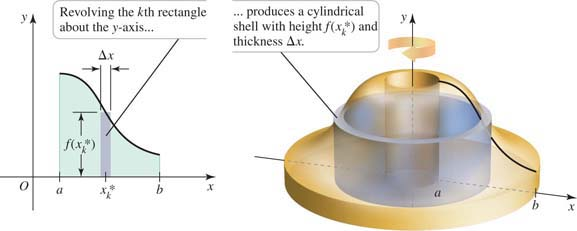
\includegraphics[width=0.6\linewidth]{../images/briggs_06_04/fig06_40}
    \vspace*{\stretch{1}}

    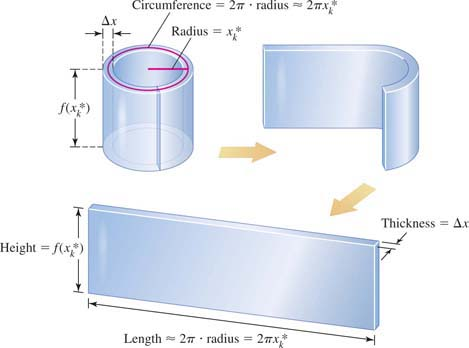
\includegraphics[width=0.5\linewidth]{../images/briggs_06_04/fig06_41}
  \end{center}
  \pagebreak

  \begin{ex*}
    Consider a general region $R$ revolved around the $y$-axis.
  \end{ex*}
  \begin{tasks}[after-item-skip=\stretch{1}, label=](1)
    \task 
      When using the \textbf{disk/washer} method, we integrate with respect to \underline{\hspace*{25mm}}
    \task 
      When using the \textbf{shell} method, we integrate with respect to \underline{\hspace*{25mm}}
  \end{tasks}
  \vspace*{\stretch{1}}
  \begin{ex*}
    Consider a general region $R$ revolved around the $x$-axis.
  \end{ex*}
  \begin{tasks}[after-item-skip=\stretch{1}, label=](1)
    \task 
      When using the \textbf{disk/washer} method, we integrate with respect to \underline{\hspace*{25mm}}
    \task 
      When using the \textbf{shell} method, we integrate with respect to \underline{\hspace*{25mm}}
  \end{tasks}
  \vspace*{\stretch{1}}
  \pagebreak

  \begin{ex*}
    Consider the region bounded between $y=x^3$, $y=8$ and $x=0$.
  \end{ex*}
  \begin{flushright}
    \begin{tikzpicture}
      \begin{axis}[
        grid style={line width=0.3pt, draw=gray!60},
        axis lines=center,
        axis line style={black,->},
        xmin=-2.5, xmax=2.5,
        ymin=-9, ymax=12,
        ymajorticks=false,
        ticklabel style={font=\footnotesize,inner sep=0.5pt,fill=white,opacity=0.5, text opacity=1},
        every axis plot/.append style={line width=0.95pt, color=blue, samples=100},
        width=0.45\linewidth, height=0.3\linewidth
        ]
        \addplot[->, name path=A, ClemsonPurple] expression[domain=-2:2.1]{x^3} node[black, pos=0.8, right, font=\normalsize] {$x^3$};
        \addplot[->, name path=B, ClemsonPurple] [domain=-2.5:2.5] {8} node[black, pos=0.25, above, font=\normalsize] {$y=8$};
        \addplot[fill=HowardsRock!55, opacity=0.75] fill between[of=A and B, soft clip={domain=0:2}];
      \end{axis}
    \end{tikzpicture}
  \end{flushright}
  \begin{tasks}[after-item-skip=\stretch{1}, label=](1)
    \task 
      Use the disk/washer method to setup the integral that represents the volume of the solid generated by rotating the region about the $x$-axis.
    \task 
      about the $y$-axis.
    \task 
      Use the disk/washer method to setup the integral that represents the volume of the solid generated by rotating the region about the line $x=-1$.
    \task 
      about the line $y=8$.
  \end{tasks}
  \vspace*{\stretch{1}}
  \pagebreak

\begin{ex*}
    Consider the region $R$ bounded by $y=4-x^2$, $y=2$, and $x=1$. Use the shell method to setup the integral that represents the volume of the solid generated by rotating the region $R$ about the indicated axis of rotation.
  \end{ex*}
  \newcommand{\parabolicFig}{
    \begin{flushright}
      \vspace*{-\baselineskip}
      \begin{tikzpicture}[scale=0.925]
        \begin{axis}[
          grid style={line width=0.3pt, draw=gray!60},
          axis lines=center,
          axis line style={black,->},
          xmin=-2.7, xmax=2.7,
          ymin=-1, ymax=4.5,
          ymajorticks=false,
          ticklabel style={font=\footnotesize,inner sep=0.5pt,fill=white,opacity=0.5, text opacity=1},
          every axis plot/.append style={line width=0.95pt, color=blue, samples=100},
          width=0.45\linewidth, height=0.3\linewidth
          ]
          \addplot[->, name path=A, ClemsonPurple] expression[domain=-2.5:2.5]{4-x^2} node[black, pos=0.71, right, font=\normalsize, xshift=-2pt] {$4-x^2$};
          \addplot[-, name path=B, ClemsonOrange] [domain=-2.5:2.5] {2} node[black, pos=0.4, above, font=\normalsize] {$y=2$};
          \addplot[fill=HowardsRock!55, opacity=0.75] fill between[of=A and B, soft clip={domain=1:1.414}];
          \draw[ClemsonOrange] (axis cs: 1,-2)--(axis cs: 1,5);
        \end{axis}
      \end{tikzpicture}
    \end{flushright}
    }
  
  \begin{tasks}[after-item-skip=\stretch{1}, label=](1)
    \task 
      about $x$-axis,
      \parabolicFig
    \task 
      about $y$-axis,
      \parabolicFig
    \task 
      about the line $x=-2$,
      \parabolicFig
    \task 
      about the line $y=2$.
      \parabolicFig
  \end{tasks}
  \pagebreak

  \begin{ex*}
    Consider the region bounded by $y=\dfrac{1}{x+1}$ and $y=1-\dfrac{x}{3}$. Use both the disk/washer method and shell method to find the volume of the solid generated when $R$ is rotated about the $x$-axis.
  \end{ex*}
  \vspace*{\stretch{1}}
  \pagebreak

  \begin{ex*}
    Determine if the following statements are true.
  \end{ex*}
  \begin{tasks}[after-item-skip=\stretch{1}, label=](1)
    \task 
      When using the shell method, the axis of the cylindrical shells is parallel to the axis of revolution.
    \task 
      If a region is revolved about the $y$-axis, then the shell method must be used.
    \task 
      If a region is revolved about the $x$-axis, it is possible to use the disk/washer method and integrate with respect to $x$.
  \end{tasks}
  \vspace*{\stretch{1}}
  \pagebreak

\end{document}

%  \documentclass[answers]{exam}
\usepackage{texPreamble}
\usepackage{relsize}
\usepackage{tabularx}
\extraheadheight{0.25in}
\extrafootheight{1.0in}
\extrawidth{1in}
% ----------------------------------------------------------------

\begin{document}
%\relscale{1.4}

\end{document}

%  \documentclass[../mathNotesPreamble]{subfiles}
\begin{document}
%  \relscale{1.4}
  \section{6.6: Surface Area}

  \begin{defn*}[Area of a Surface of Revolution]
    Let $f$ be a nonnegative function with a continuous first derivative on the interval $\sbrkt{a,b}$. The area of the surface generated when the graph of $f$ on the interval $\sbrkt{a,b}$ is revolved around the $x$-axis is
      \[S=\int_a^b 2\pi f(x)\sqrt{1+f'(x)^2}\,dx.\]
  \end{defn*}

  \begin{center}
    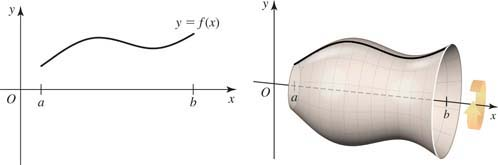
\includegraphics[width=0.5\linewidth]{../images/briggs_06_06/fig06_60}
  \end{center}

  \begin{ex*}
    Find the exact area of the surface obtained by rotating the curve $y=x^3$, $0\leq x\leq 2$ about the $x$-axis.
  \end{ex*}
  \vspace*{\stretch{1}}
  \pagebreak

  \begin{ex*}
    Find the exact area of the surface obtained by rotating the curve $y=\sqrt{8x-x^2}$, $1\leq x\leq 7$ about the $x$-axis.
  \end{ex*}
  \vspace*{\stretch{1}}
  \pagebreak

  \begin{ex*}
    Find the exact area of the surface obtained by rotating the curve $y=\dfrac{1}{2}\parens{e^{x}+e^{-x}}$, $-\ln(2)\leq x\leq \ln(2)$ about the $x$-axis.
  \end{ex*}
  \vspace*{\stretch{1}}
  \pagebreak

  

\end{document}

%  \documentclass[../mathNotesPreamble]{subfiles}
\begin{document}
  \relscale{1.4}
  \section*{6.7: Physical Applications}

  \begin{defn*}[Mass of a One-Dimensional Object]
    Suppose a thin bar or wire is represented by the interval $a\leq x\leq b$ with a density function $\rho$ (with units of mass per length). The \textbf{mass} of the object is
      \[m=\int_a^b \rho(x)\,dx.\]
  \end{defn*}

  \begin{defn*}[Work]
    The work done by a variable force $F$ moving an object along a line from $x=a$ to $x=b$ in the direction of the force is
      \[W=\int_a^b F(x)\,dx.\]
  \end{defn*}

  %TODO Hooke's law

  \begin{thmBox*}[Procedure: Solving Pumping Problems]
    \begin{enumerate}
      \item 
        Draw a $y$-axis in the vertical direction (parallel to gravity) and choose a convenient origin. Assume the interval $\sbrkt{a,b}$ corresponds to the vertical extent of the fluid.
      \item 
        For $a\leq y\leq b$, find the cross-sectional area $A(y)$ of the horizontal slices and the distance $D(y)$ the slices must be lifted.
      \item 
        The work required to lift the water is
          \[W=\int_a^b \rho gA(y)D(y)\,dy.\]
    \end{enumerate}
  \end{thmBox*}

  \begin{thmBox*}[Procedure: Solving Force-on-Dam Problems]
    \begin{enumerate}
      \item 
        Draw a $y$-axis on the face of the dam in the vertical direction and choose a convenient origin (often taken to be the base of the dam).
      \item 
        Find the width function $w(y)$ for each value of $y$ on the face of the dam.
      \item 
        If the base of the dam is at $y=0$ and the top of the dam is at $y=a$, then the total force on the dam is
          \[F=\int_a^b \rho g\underbrace{(a-y)}_{\textnormal{depth}}\underbrace{w(y)}_{\textnormal{width}}\,dy.\]
    \end{enumerate}
  \end{thmBox*}

\end{document}

%  \documentclass[answers]{exam}
\usepackage{texPreamble}
\usepackage{relsize}
\usepackage{tabularx}
\extraheadheight{0.25in}
\extrafootheight{1.0in}
\extrawidth{1in}
% ----------------------------------------------------------------

\begin{document}
%\relscale{1.4}

\end{document}

%  \documentclass[answers]{exam}
\usepackage{texPreamble}
\usepackage{relsize}
\usepackage{tabularx}
\extraheadheight{0.25in}
\extrafootheight{1.0in}
\extrawidth{1in}
% ----------------------------------------------------------------

\begin{document}
%\relscale{1.4}

\end{document}

%  \documentclass[answers]{exam}
\usepackage{texPreamble}
\usepackage{relsize}
\usepackage{tabularx}
\extraheadheight{0.25in}
\extrafootheight{1.0in}
\extrawidth{1in}
% ----------------------------------------------------------------

\begin{document}
%\relscale{1.4}

\end{document}

%  \documentclass[answers]{exam}
\usepackage{texPreamble}
\usepackage{relsize}
\usepackage{tabularx}
\extraheadheight{0.25in}
\extrafootheight{1.0in}
\extrawidth{1in}
% ----------------------------------------------------------------

\begin{document}
%\relscale{1.4}

\end{document}

%  \documentclass[../mathNotesPreamble]{subfiles}
\begin{document}
%  \relscale{1.4}
  \section{8.5: Partial Fractions}
  \begin{ex*}
    Simplify $\displaystyle f(x)=\frac{1}{x-2}+\frac{2}{x+4}$ by finding a common denominator.
  \end{ex*}
  \vspace*{\stretch{0.5}}

  \begin{thmBox*}[Procedure: Partial Fractions with Simple Linear Factors]
    Suppose $f(x)=p(x)/q(x)$, where $p$ and $q$ are polynomials with no common factors and with the degree of $P$ less than the degree of $q$. Assume $q$ is the product of simple linear factors. The partial fraction decomposition is obtained as follows.
    \begin{enumerate}[label=\textbf{Step \arabic*:}, itemindent=1.5\labelwidth]
      \item \textbf{Factor the denominator $q$} in the form $(x-r_1)(x-r_2)\dots(x-r_n)$
      \item \textbf{Partial fraction decomposition}
        \[\frac{p(x)}{q(x)}=\frac{A_1}{(x-r_1)}+\frac{A_2}{(x-r_2)}+\dots+\frac{A_n}{(x-r_n)}.\]
      \item \textbf{Clear denominators} Multiply both sides of the equation in Step 2 by $q(x)=(x-r_1)(x-r_2)\dots(x-r_n)$
      \item \textbf{Solve for coefficients} Equate like powers of $x$ in Step 3 to solve for the undetermined coefficients $A_1,\dots,A_n$.
    \end{enumerate}
  \end{thmBox*}

  \begin{ex*}
    Perform partial fraction decomposition on $\displaystyle f(x)=\frac{3x}{x^2+2x-8}$.
  \end{ex*}
  \vspace*{\stretch{1}}
  \pagebreak

  \begin{ex*}
    $\displaystyle \int \frac{28x^3-56x^2+9}{x^2-2x}$
  \end{ex*}
  \vspace*{\stretch{1}}
  \pagebreak

  \begin{thmBox*}[Procedure: Partial Fractions for Repeated Linear Factors]
    Suppose the repeated linear factor $(x-r)^m$ appears in the denominator of a proper rational function in reduced form. The partial fraction decomposition has a partial fraction for each power of $(x-r)$ up to and including the $m$th power; that is, the partial fraction decomposition contains the sum  
    \[\frac{A_1}{(x-r)}+\frac{A_3}{(x-r)^2}+\frac{A_3}{(x-r)^3}+\dots+\frac{A_m}{(x-r)^m}\]
    where $A_1,\dots,A_m$ are constants to be determined.
  \end{thmBox*}
  \begin{ex*}
    Setup the partial fraction decomposition for $\displaystyle f(x)=\frac{x^3-8x+19}{x^4+3x^3}$.
  \end{ex*}
  \vspace*{\stretch{1}}
  \begin{ex*}
    Setup the partial fraction decomposition for $\displaystyle g(x)=\frac{2}{x^5-6x^4+9x^3}$.
  \end{ex*}
  \vspace*{\stretch{1}}
  \pagebreak

  \begin{ex*}
    Evaluate $\displaystyle \int \frac{x^2+1}{(2x-3)(x-2)^2}\,dx$.
  \end{ex*}
  \vspace*{\stretch{1}}
  \pagebreak

  \begin{ex*}
    Evaluate $\displaystyle \int \frac{8}{3x^3+7x2+4x}\,dx$.
  \end{ex*}
  \vspace*{\stretch{1}}
  \pagebreak

  \begin{ex*}
    Perform partial fraction decomposition on the following fractions or identify them as irreducible.
  \end{ex*}
  \begin{tasks}[after-item-skip=\stretch{1}, label=, item-indent=0mm](1)
    \task $\displaystyle \frac{1}{x^2-13x+43}$
    \task $\displaystyle \frac{x^2}{(x-4)(x+5)}$
  \end{tasks}
  \vspace*{\stretch{1}}
  \pagebreak

  \begin{ex*}
    Perform partial fraction decomposition on the following fractions or identify them as irreducible.
  \end{ex*}
  \begin{tasks}[after-item-skip=\stretch{1}, label=, item-indent=0mm](1)
    \task $\displaystyle \frac{7}{(x^2+1)^2}$
    \task $\displaystyle \frac{1}{x^2+11x+28}$
  \end{tasks}
  \vspace*{\stretch{1}}
  \pagebreak

  \begin{ex*}
    Evaluate $\displaystyle \int \frac{4x}{(x+1)(x^2+1)}\,dx$
  \end{ex*}
  \vspace*{\stretch{1}}
  \pagebreak

  \begin{ex*}
    Evaluate $\displaystyle \int \frac{3x^2+2x+12}{(x^2+4)^2}\,dx$
  \end{ex*}
  \vspace*{\stretch{1}}
  \pagebreak

  \begin{ex*}
    Evaluate $\displaystyle \int \frac{1}{x\sqrt{1+2x}}\,dx$ using the substitution $u=\sqrt{1+2x}$.
  \end{ex*}
  \vspace*{\stretch{1}}
  \pagebreak

\end{document}

%  \documentclass[answers]{exam}
\usepackage{texPreamble}
\usepackage{relsize}
\usepackage{tabularx}
\extraheadheight{0.25in}
\extrafootheight{1.0in}
\extrawidth{1in}
% ----------------------------------------------------------------

\begin{document}
%\relscale{1.4}

\end{document}

%  \documentclass[../mathNotesPreamble]{subfiles}
\begin{document}
%  \relscale{1.4}
  \section{8.9: Improper Integrals}
    \begin{defn*}[Improper Integrals over Infinite Intervals]
      \begin{enumerate}
        \item \label{infInterval_case1} If $f$ is continuous on $[a,\infty)$, then
          \[\int_a^\infty f(x)\,dx=\lim_{b\to \infty} \int_a^b f(x)\,dx.\]
        \item \label{infInterval_case2} If $f$ is continuous on $(-\infty,b]$, then
          \[\int_{-\infty}^b f(x)\,dx=\lim_{a\to -\infty} \int_a^b f(x)\,dx.\]
        \item \label{infInterval_case3} If $f$ is continuous on $(-\infty,\infty)$, then
          \[\int_{-\infty}^\infty f(x)\,dx=\lim_{a\to-\infty}\int_a^c f(x)\,dx+\lim_{b\to\infty}\int_c^b f(x)\,dx.\]
          where $c$ is any real number. It can be shown that the choice of $c$ does not affect the value or convergence of the original integral.
      \end{enumerate}
      If the limits in cases \ref{infInterval_case1}-- \ref{infInterval_case3} exist, then the improper integrals \textbf{converge}; otherwise they \textbf{diverge}.
    \end{defn*}

    \begin{ex*}
      Evaluate $\displaystyle \int_1^\infty \frac{\ln(x)}{x}\,dx$ and determine if the integral converges or diverges.
    \end{ex*}
    \vspace*{\stretch{1}}
    \pagebreak

    \begin{ex*}
      Evaluate $\displaystyle \int_{-\infty}^{\infty} \frac{e^{3x}}{1+e^{6x}}\,dx$.
    \end{ex*}
    \vspace*{\stretch{1}}
    \pagebreak

    \begin{ex*}
      For what values of $p$ does $\displaystyle \int_1^\infty \frac{1}{x^p}\,dx$ converge?
    \end{ex*}
    \vspace*{\stretch{1}}
    \pagebreak

    \begin{defn*}[Improper Integrals with Unbounded Integrand]
      \begin{enumerate}
        \item \label{unboundedIntegrand_case1} Suppose $f$ is continuous on $(a,b]$ with $\displaystyle \lim_{x\to a^+} f(x)=\pm\infty$. Then
          \[\int_a^b f(x)\,dx=\lim_{c\to a^+} \int_c^b f(x)\,dx.\]
        \item \label{unboundedIntegrand_case2} Suppose $f$ is continuous on $[a,b)$ with $\displaystyle \lim_{x\to b^-} f(x)=\pm\infty$. Then
          \[\int_a^b f(x)\,dx=\lim_{c\to b^-} \int_a^c f(x)\,dx.\]
        \item \label{unboundedIntegrand_case3} Suppose $f$ is continuous on $[a,b]$ except at the interior point $p$ where $f$ is unbounded. Then
          \[\int_a^b f(x)\,dx=\lim_{c\to p^-} \int_a^c f(x)\,dx + \lim_{d\to p^+}\int_d^b f(x)\,dx.\]
      \end{enumerate}
      If the limits in cases \ref{unboundedIntegrand_case1}-- \ref{unboundedIntegrand_case3} exist, then the improper integrals \textbf{converge}; otherwise, they \textbf{diverge}.
    \end{defn*}
    \pagebreak

    \begin{ex*}
      Determine which of the following integrals are improper integrals
    \end{ex*}
    \begin{tasks}[after-item-skip=\stretch{1}, label=, item-indent=0pt](2)
      \task $\displaystyle \int_0^1 \sec(x)\,dx$
      \task $\displaystyle \int_{\pi/2}^{3\pi/4} \tan(x)\,dx$
      \task $\displaystyle \int_1^e \ln(x)\,dx$
      \task $\displaystyle \int_0^1 \arctan(x)\,dx$
      \task $\displaystyle \int_0^{0.5} \ln(x)\,dx$
      \task $\displaystyle \int_{-10}^{-1} \frac{1}{x^{1/3}}\,dx$
    \end{tasks}
    \vspace*{\stretch{1}}
    \pagebreak

    \begin{ex*}
      Evaluate $\displaystyle \int_1^9 \frac{dx}{(x-1)^{2/3}}.$ Does this integral converge or diverge?
    \end{ex*}
    \vspace*{\stretch{1}}
    \pagebreak

    \begin{ex*}
      Evaluate $\displaystyle \int_{-1}^{1} \frac{e^{2/x}}{x^2}\,dx$. Does this integral converge or diverge?
    \end{ex*}
    \vspace*{\stretch{1}}
    \pagebreak

    \begin{thmBox*}[Theorem 8.2: Comparison Test for Improper Integrals]
      Suppose the functions $f$ and $g$ are continuous on the interval $[a,\infty)$, with\newline $f(x)\geq g(x)\geq 0$, for $x\geq a$.
      \begin{enumerate}
        \item If $\displaystyle \int_a^\infty f(x)\,dx$ converges, then $\displaystyle\int_a^\infty g(x)\,dx$ converges.
        \item If $\displaystyle \int_a^\infty g(x)\,dx$ diverges, then $\displaystyle\int_a^\infty f(x)\,dx$ diverges.
      \end{enumerate}
    \end{thmBox*}

    \begin{ex*}
      Determine if the integral $\displaystyle \int_2^\infty \frac{x^3}{x^4-x^3-1}\,dx$ converges or diverges.
    \end{ex*}
    \vspace*{\stretch{1}}
    \pagebreak

  \begin{ex*}[Gabriel's Horn]
      Let $R$ be the region bounded by the graph of $y=1/x$ and the $x$-axis for $x\geq 1$. 
    \end{ex*}
    \begin{tasks}[after-item-skip=\stretch{1}, label=, item-indent=0pt](1)
      \task What is the volume of the solid generated when $R$ is revolved around the $x$-axis?
      \task What is the surface area of the solid generated when $R$ is revolved about the $x$-axis?
    \end{tasks}
    \vspace*{\stretch{1}}
    \pagebreak

\end{document}

%  \documentclass[answers]{exam}
\usepackage{texPreamble}
\usepackage{relsize}
\usepackage{tabularx}
\extraheadheight{0.25in}
\extrafootheight{1.0in}
\extrawidth{1in}
% ----------------------------------------------------------------

\begin{document}
%\relscale{1.4}

\end{document}

%  \documentclass[../mathNotesPreamble]{subfiles}
\begin{document}
%  \relscale{1.4}
  \section{10.2: Sequences}

  \begin{thmBox*}[Theorem 10.1: Limits of Sequences from Limits of Functions]
    Suppose $f$ is a function such that $f(n)=a_n$, for positive integers $n$. If \newline$\displaystyle \lim_{x\to \infty} f(x)=L$, then the limit of the sequence $\set{a_n}$ is also $L$, where $L$ may be $\pm\infty$.
  \end{thmBox*}

  \begin{ex*}
    Determine if the following sequences converge or diverge. If the sequence converges, find its limit.
  \end{ex*}
  \begin{tasks}[after-item-skip=\stretch{1}, label=, item-indent=0pt](2)
    \task $\set{e^{2n/(n+2)}}_{n=1}^{\infty}$
    \task $\set{\frac{(-1)^n}{n}}_{n=1}^{\infty}$
    \task $\set{\frac{\arctan(n)}{n}}_{n=1}^{\infty}$
    \task $\set{\frac{e^{-n}}{42\sin(e^{-n})}}_{n=1}^{\infty}$
  \end{tasks}
  \vspace*{\stretch{1}}
  \pagebreak

  \begin{thmBox*}[10.2: Limit Laws for Sequences]
    Assume the sequences $\set{a_n}$ and $\set{b_n}$ have limits $A$ and $B$, respectively. Then
      \begin{enumerate}
        \item $\displaystyle \lim_{n\to \infty}\parens{a_n\pm b_n}=A\pm B$
        \item $\displaystyle \lim_{n\to \infty} ca_n=cA$, where $c$ is a real number
        \item $\displaystyle \lim_{n\to \infty} a_nb_n=AB$
        \item $\displaystyle \lim_{n\to \infty} \frac{a_n}{b_n}= \frac{A}{B}$, provided $B\neq0$.
      \end{enumerate}
  \end{thmBox*}

  \begin{ex*}
    Consider the sequences $\set{a_n}$, $\set{b_n}$, $\set{c_n}$, and $\set{d_n}$ where
      \[a=\frac{1}{n},\quad b_n=n,\quad c_n=e^n,\quad \textnormal{ and } d_n=\sqrt{n}.\]
    Compute the following limits.
  \end{ex*}
  \begin{tasks}[after-item-skip=\stretch{1}, label=\Alph*., item-indent=17.5pt](4)
    \task $\displaystyle \lim_{n\to \infty} a_n$
    \task $\displaystyle \lim_{n\to \infty} b_n$
    \task $\displaystyle \lim_{n\to \infty} c_n$
    \task $\displaystyle \lim_{n\to \infty} d_n$
    \task $\displaystyle \lim_{n\to \infty} a_nb_n$
    \task $\displaystyle \lim_{n\to \infty} a_nc_n$
    \task $\displaystyle \lim_{n\to \infty} a_nd_n$
  \end{tasks}
  \vspace*{\stretch{1}}


  \noindent
  True or False: If for some sequence $\set{a_n}$ and $\set{b_n}$, $\displaystyle\lim_{n\to \infty}a_n=0$ and $\displaystyle\lim_{n\to \infty} b_n=\infty$, then $\displaystyle\lim_{n\to \infty} a_nb_n=0$.
  \pagebreak

  \begin{defn*}[Terminology for Sequences]
    \begin{enumerate}[label=\textbullet, itemsep=15pt]
      \item $\set{a_n}$ is \textbf{increasing} if $a_{n+1}>a_n$
      \item $\set{a_n}$ is \textbf{nondecreasing} if $a_{n+1}\geq a_n$
      \item $\set{a_n}$ is \textbf{decreasing} if $a_{n+1}< a_n$
      \item $\set{a_n}$ is \textbf{nonincreasing} if $a_{n+1}\leq a_n$
      \item $\set{a_n}$ is \textbf{monotonic} if it is either nonincreasing or nondecreasing (it moves in one direction)
      \item $\set{a_n}$ is \textbf{bounded above} if there is a number $M$ such that $a_n\leq M$, for all relevant values of $n$
      \item $\set{a_n}$ is \textbf{bounded below} if there is a number $N$ such that $a_n\geq N$, for all relevant values of $n$.
      \item If $\set{a_n}$ is bounded above and bounded below, then we say that $\set{a_n}$ is a \textbf{bounded} sequence.
    \end{enumerate}
  \end{defn*}
  \begin{ex*}
    Consider the sequence $\set{-n^2}_{n=1}^{\infty}$. What can we say about this sequence?
  \end{ex*}
  \vspace*{\stretch{1}}
  \pagebreak

  \begin{thmBox*}[Theorem 10.3: Geometric Sequences]
    Let $r$ be a real number. Then
      \[\lim_{n\to \infty} r^n =
        \begin{cases}
          0&\textnormal{ if } \abs{r}<1\\
          1&\textnormal{ if } r=1\\
          \textnormal{does not exist}& \textnormal{ if } r\leq -1 \textnormal{ or } r>1.
        \end{cases}
      \]
      If $r>0$, then $\set{r^n}$ is a monotonic sequence. If $r<0$, then $\set{r^n}$ oscillates.

      \begin{center}
        \begin{tikzpicture}[scale=2]
          \begin{axis}[
            axis line style={<->},
            xticklabel style = {yshift=-2pt},
            axis y line=none,
            axis x line*=center,
            ymin=0, ymax=1,
            xmin=-3, xmax=3,
            width=0.5\textwidth, height=24mm,
            xtick={-1,0,1},
            ticklabel style={font=\scriptsize,fill=white,opacity=1.0, text opacity=1},
            xlabel=$r$, xlabel style={at={(ticklabel* cs: 1.0), font=\normalsize}, below}
            ]
            \addplot[holdot, draw=black] coordinates{(-1,0)};
            \addplot[soldot, black] coordinates{(1,0)};
            \fill[ClemsonOrange, opacity=0.5] (-1,0) -- (1,0) -- (1,1) -- (-1,1) -- cycle;
            \fill[left color=white, right color=ClemsonPurple, opacity=0.25] (-2.75,0) -- (-1,0) -- (-1,1) -- (-2.75,1) -- cycle;
            \fill[right color=white, left color=ClemsonPurple, opacity=0.25] (2.75,0) -- (1,0) -- (1,1) -- (2.75,1) -- cycle;
            \draw[densely dashed, line width=0.75pt] (-1,0) -- (-1,1);
            \draw[line width=0.75pt] (1,0) -- (1,1);
            \node[font=\scriptsize, align=center] at (axis cs: -1.8,0.5) {Diverges\\ $r\leq -1$};
            \node[font=\scriptsize, align=center] at (axis cs: 0,0.5) {Converges\\ $-1<r\leq 1$};
            \node[font=\scriptsize, align=center] at (axis cs: 1.8,0.5) {Diverges\\ $r> 1$};
          \end{axis}
        \end{tikzpicture}
      \end{center}
    \vspace*{-\baselineskip}
  \end{thmBox*}

  \begin{ex*}
    Determine if the following sequences converge
  \end{ex*}
  \begin{tasks}[after-item-skip=\stretch{1}, label=, item-indent=0pt](2)
    \task $\displaystyle \set{\frac{3^{n+1}+3}{3^n}}$
    \task $\displaystyle \set{2^{n+1}3^{-n}}$
    \task $\displaystyle \set{\frac{(-1)^n}{2^n}}$
    \task $\displaystyle \set{\frac{75^{n-1}}{99^n}+\frac{5^n\sin(n)}{8^n}}$
  \end{tasks}
  \vspace*{\stretch{1}}
  \pagebreak

  \begin{thmBox*}[Theorem 10.4: Squeeze Theorem for Sequences]
    Let $\set{a_n}$, $\set{b_n}$, and $\set{c_n}$ be sequences with $a_n\leq b_n\leq c_n$, for all integers $n$ greater than some index $N$. If $\displaystyle\lim_{n\to \infty} a_n=\lim_{n\to \infty} c_n=L$, then $\displaystyle\lim_{n\to \infty} b_n=L$.
  \end{thmBox*}
  \begin{ex*}
    Find the limit of the sequence $b_n=\dfrac{9\cos(n)}{n^2+1}$.
  \end{ex*}
  \vspace*{\stretch{1}}

  \begin{thmBox*}[Theorem 10.5: Bounded Monotonic Sequence]
    A bounded monotonic sequence converges.
  \end{thmBox*}
  \pagebreak

  \begin{thmBox*}[Theorem 10.6: Growth Rates of Sequences]
    The following sequences are ordered according to increasing growth rates as $n\to\infty$; that is, if $\set{a_n}$ appears before $\set{b_n}$ in the list, then $\displaystyle\lim_{n\to \infty} \frac{a_n}{b_n}=0$ and $\displaystyle\lim_{n\to \infty} \frac{b_n}{a_n}=\infty$:
      \[\set{\parens{\ln n}^q} \hspace*{2.5pt} \ll \hspace*{2.5pt} \set{n^p} \hspace*{2.5pt} \ll \hspace*{2.5pt} \set{n^p\parens{\ln n}^r} \hspace*{2.5pt} \ll \hspace*{2.5pt} \set{n^{p+s}} \hspace*{2.5pt} \ll \hspace*{2.5pt} \set{b^n} \hspace*{2.5pt} \ll \hspace*{2.5pt} \set{n!} \hspace*{2.5pt} \ll \hspace*{2.5pt} \set{n^n}\]
  \end{thmBox*}

  \begin{ex*}
    Use growth rates to determine which of the following sequences converge.
  \end{ex*}
  \begin{tasks}[after-item-skip=\stretch{1}, label=,item-indent=0pt](1)
    \task $\displaystyle\set{\frac{\ln(n^{10})}{0.00001n}}$
    \task $\displaystyle\set{\frac{n^8\ln(n)}{n^{8.001}}}$
    \task $\displaystyle\set{\frac{n!}{10^n}}$
  \end{tasks}
  \vspace*{\stretch{1}}
  \pagebreak

  \begin{defn*}[Limit of a Sequence]
    The sequence $\set{a_n}$ converges to $L$ provided the terms of $a_n$ can be made arbitrarily close to $L$ by taking $n$ sufficiently large. More precisely, $\set{a_n}$ has the unique limit $L$ if, given any $\eps >0$, it is possible to find a positive integer $N$ (depending only on $\eps$) such that
      \[\abs{a_n-L}< \eps \qquad \textnormal{ whenever } n>N.\]
    If the \textbf{limit of a sequence} is $L$, we say the sequence \textbf{converges} to $L$, written
      \[\lim_{n\to \infty} a_n=L.\]
    A sequence that does not converge is said to \textbf{diverge}.
  \end{defn*}
  \vspace*{\stretch{1}}

\pagebreak
\end{document}

%  \documentclass[answers]{exam}
\usepackage{texPreamble}
\usepackage{relsize}
\usepackage{tabularx}
\extraheadheight{0.25in}
\extrafootheight{1.0in}
\extrawidth{1in}
% ----------------------------------------------------------------

\begin{document}
%\relscale{1.4}

\end{document}

%  \documentclass[answers]{exam}
\usepackage{texPreamble}
\usepackage{relsize}
\usepackage{tabularx}
\extraheadheight{0.25in}
\extrafootheight{1.0in}
\extrawidth{1in}
% ----------------------------------------------------------------

\begin{document}
%\relscale{1.4}

\end{document}

%  \documentclass[answers]{exam}
\usepackage{texPreamble}
\usepackage{relsize}
\usepackage{tabularx}
\extraheadheight{0.25in}
\extrafootheight{1.0in}
\extrawidth{1in}
% ----------------------------------------------------------------

\begin{document}
%\relscale{1.4}

\end{document}

%  \documentclass[../mathNotesPreamble]{subfiles}
\begin{document}
%  \relscale{1.4}
  \section{10.6: Alternating Series}

  \begin{thmBox*}[Theorem 10.16: Alternating Series Test]
    The alternating series $\sum(-1)^{k+1}a_k$ converges provided
    \begin{enumerate}
      \item the terms of the series are nonincreasing in magnitude $(0< a_{k+1}\leq a_k$, for $k$ greater than some index $N$) and
      \item $\displaystyle \lim_{k\to \infty} a_k=0$.
    \end{enumerate}
  \end{thmBox*}
  \begin{ex*}
    Which of the following are considered alternating series?
  \end{ex*}
  \begin{tasks}[after-item-skip=\stretch{1}, label=,item-indent=0pt](4)
    \task $\displaystyle \sum_{k=0}^\infty \frac{(-1)^{k+1}}{k+2}$
    \task $\displaystyle \sum_{k=4}^\infty \parens{\frac{-3}{2}}^k$
    \task $\displaystyle \sum_{k=0}^\infty (-1)\parens{\frac{1}{2}}^k$
    \task $\displaystyle \sum_{k=1}^\infty (-1)^{k+1}\parens{\frac{1}{2}}^k$
    \task $\displaystyle \sum_{k=-3}^\infty \frac{\cos(k\pi)}{(k+4)^2}$
    \task $\displaystyle \sum_{k=1}^\infty \frac{\sin(k)}{k^2}$
    \task $\displaystyle \sum_{k=0}^\infty (-1)^{k+1}\parens{\frac{1}{-2}}^k$
  \end{tasks}
  \vspace*{\stretch{1}}
  \pagebreak

  \begin{ex*}
    Consider the series $\displaystyle\sum_{k=1}^\infty (-1)^k \frac{\sqrt{k}}{2k+3}$. Let $a_k$ represent that magnitude of the terms of the given series.
  \end{ex*}
  \begin{tasks}[after-item-skip=\stretch{1}, label=\textbullet,item-indent=0pt](1)
    \task What is $\displaystyle\lim_{k\to \infty} a_k$?
    \task Compute $f'(x)$ where $f(k)=a_k$.
    \task Use the Alternating Series Test to determine if the given series converges.
  \end{tasks}
  \vspace*{\stretch{1}}
  \pagebreak

  \begin{ex*}
    Does the series $\displaystyle\sum_{k=0}^\infty (-1)^{k+1}\parens{\frac{4}{3}}^k$ converge?
  \end{ex*}
  \vspace*{\stretch{1}}

  \begin{ex*}
    Does the series $\displaystyle\sum_{k=1}^\infty \cos(\pi k)e^{-k}$ converge? 
  \end{ex*}
  \vspace*{\stretch{1}}
  \pagebreak

  \begin{thmBox*}[Theorem 10.17: Alternating Harmonic Series]
    The alternating harmonic series $\displaystyle\sum_{k=1}^\infty \frac{(-1)^{k+1}}{k}$ converges (even though the harmonic series $\displaystyle\sum_{k=1}^\infty \frac{1}{k}$ diverges).
  \end{thmBox*}
  \begin{ex*}
    Use the Alternating Series Test to show that the alternating harmonic series converges.
  \end{ex*}
  \vspace*{\stretch{1}}
  \pagebreak

  \begin{thmBox*}[Theorem 10.18: Remainder in Alternating Series]
    Let $\displaystyle\sum_{k=1}^\infty (-1)^{k+1} a_k$ be a convergent alternating series with terms that are nonincreasing in magnitude. Let $R_n=S-S_n$ be the remainder in approximating the value of that series  by the sum of its first $n$ terms. Then $\abs{R_n}\leq a_{n+1}$. In other words, the magnitude of the remainder is less than or equal to the magnitude of the first neglected term.
  \end{thmBox*}

  

  \noindent
  \begin{minipage}[t]{0.6\linewidth}
    \begin{ex*}
      Find the minimum value of $n$ such that $\abs{R_n}< 10^{-4}$ for the following series:
    \end{ex*}
      \[\ln(2)=\sum_{k=1}^\infty \frac{(-1)^{k+1}}{k}\]
  \end{minipage}%
  \begin{minipage}[t]{0.4\linewidth}
    \mbox{}\vspace*{-1.5\baselineskip}
    \begin{flushright}
      \begin{tikzpicture}[
        declare function={S=3; 
        n=1.75;   Sn=4.5;
        npo=4.75; Snpo=2.25;}]
        \begin{axis}[
          major grid style={line width=0.375pt, draw=gray!75},
          axis lines=center,
          axis line style={black,->},
          xmin=-0.5, xmax=6,
          ymin=-0.5, ymax=6,
          xtick={n,npo},
          xticklabels={$n$,$n+1$},
          ytick={S},
          yticklabels={$S$},
          ticklabel style={font=\normalsize,inner sep=0.5pt,fill=white,opacity=1.0, text opacity=1},
          ylabel=$S_n$, ylabel style={at={(ticklabel* cs:1)},anchor=south west},
          every axis plot/.append style={line width=0.95pt, color=blue, samples=100}
          ]
          \addplot[dashed] expression[domain=0:6]{S};
          \addplot[soldot,red] coordinates{(n,Sn)} node[above, black, font=\large] {$S_n$};
          \addplot[soldot,red] coordinates{(npo,Sn)} node[above, black, font=\large] {$S_n$};
          \addplot[soldot,red] coordinates{(npo,Snpo)} node[below, black, font=\large] {$S_{n+1}$};
          \draw[<->, shorten < = 2pt] (n,Sn) -- node[font=\scriptsize, fill=white, inner sep=1.5pt] {$\abs{R_n}=\abs{S-S_n}$} (n,S) ;
          \draw[<->, shorten > = 2pt, shorten < = 2pt] (npo,Sn) -- node[font=\scriptsize, fill=white, inner sep=1.5pt] {$\abs{S_n-S_{n+1}}$} (npo,Snpo);
          \node[font=\normalsize, draw=black!50, rounded corners] at (3.5,0.75) {$\abs{R_n}\leq \abs{S_{n+1}-S_n}=a_{n+1}$};
        \end{axis}
      \end{tikzpicture}
    \end{flushright}
  \end{minipage}
  \vspace*{\stretch{1}}
  \pagebreak

  \begin{defn*}[Absolute and Conditional Convergence]
    If $\sum\abs{a_k}$ converges, then $\sum a_k$ \textbf{converges absolutely}.\newline
    If $\sum\abs{a_k}$ diverges and $\sum a_k$ converges, then $\sum a_k$ \textbf{converges conditionally}.
  \end{defn*}
  \begin{ex*}
    Can a series of strictly positive terms converge conditionally?
  \end{ex*}
  \vspace*{\stretch{0.25}}
  \begin{ex*}
    Consider the series $\displaystyle\sum_{k=1}^\infty (-1)^{k+1}\frac{4+k}{k^2}$. Determine if this series converges absolute, converges conditionally, or diverges.
  \end{ex*}
  \vspace*{\stretch{1}}
  \pagebreak

  \begin{ex*}
    Determine if the following series converge absolute, converge conditionally, or diverge.
  \end{ex*}
  \begin{tasks}[after-item-skip=\stretch{1}, label=,item-indent=0pt](1)
    \task $\displaystyle\sum_{k=1}^\infty \frac{(-1)^{k+1}}{2\sqrt{k}-1}$
    \task $\displaystyle\sum_{k=1}^\infty \parens{\frac{3}{4}}^k$
  \end{tasks}
  \vspace*{\stretch{1}}
  \pagebreak

  \begin{thmBox*}[Theorem 10.19: Absolute Convergence Implies Convergence]
    If $\sum \abs{a_k}$ converges, then $\sum a_k$ converges (absolute convergence implies convergence). Equivalently, if $\sum a_k$ diverges, then $\sum\abs{a_k}$ diverges.
  \end{thmBox*}
  \begin{ex*}
    Determine whether each of the following series converges absolutely, converges conditionally or diverges.
  \end{ex*}
  \begin{tasks}[after-item-skip=\stretch{1}, label=,item-indent=0pt](1)
    \task $\displaystyle\sum_{k=1}^\infty (-1)^ke^{1/k}$
    \task $\displaystyle\sum_{k=1}^\infty \frac{(-1)^{k+1}}{k^6}$
  \end{tasks}
  \vspace*{\stretch{1}}
  \pagebreak

  \begin{tasks}[after-item-skip=\stretch{1}, label=,item-indent=0pt](1)
    \task $\displaystyle\sum_{k=1}^\infty \frac{(-1)^k}{3^k}$
    \task $\displaystyle\sum_{k=1}^\infty \frac{(-5)^k}{3^k}$
    \task $\displaystyle\sum_{k=1}^\infty \frac{(-2)^{k-1}}{3^k}$
  \end{tasks}
  \vspace*{\stretch{1}}
  \pagebreak

  \begin{ex*}
    Does the series $\displaystyle\sum_{k=1}^\infty \frac{1}{2\sqrt{k}-1}$ converge conditionally, converge absolutely, or diverge?
  \end{ex*}
  \vspace*{\stretch{1}}
  \pagebreak

\end{document}
%  \documentclass[answers]{exam}
\usepackage{texPreamble}
\usepackage{relsize}
\usepackage{tabularx}
\extraheadheight{0.25in}
\extrafootheight{1.0in}
\extrawidth{1in}
% ----------------------------------------------------------------

\begin{document}
%\relscale{1.4}

\end{document}

%  \documentclass[../mathNotesPreamble]{subfiles}
\begin{document}
%\relscale{1.4}
  \section*{10.8: Choosing a Convergence Test}

  \begin{ex*}
    Consider the series $\displaystyle\sum_{k=1}^\infty \frac{(-1)^{k+1}}{k}$. Is this series conditionally convergent, absolutely convergent, or divergent? Which test do you use?
  \end{ex*}
  \vspace*{\stretch{1}}
  \pagebreak

  \begin{ex*}
    Consider the series $\displaystyle\sum_{k=1}^\infty \frac{(-1)^{k+1}}{k^2}$. Is this series conditionally convergent, absolutely convergent, or divergent? Which test do you use?
  \end{ex*}
  \vspace*{\stretch{1}}
  \pagebreak

  \begin{ex*}
    Which of the following series can be rewritten as a $p$-series?
  \end{ex*}
  \begin{tasks}[after-item-skip=\stretch{1}, label=,item-indent=0pt](2)
    \task $\displaystyle\sum_{k=1}^\infty \frac{(-1)^{2k}}{k\sqrt{k}}$
    \task $\displaystyle\sum_{k=1}^\infty \frac{(-1)^k}{k^5}$
    \task $\displaystyle\sum_{k=1}^\infty \frac{k^2+k+1}{k^4+2}$
    \task $\displaystyle\sum_{k=1}^\infty \frac{3^k}{k^4}$
    \task $\displaystyle\sum_{k=1}^\infty \frac{\sqrt{k}}{k^2}$
  \end{tasks}
  \vspace*{\stretch{1}}
  \pagebreak

  \begin{ex*}
    Which test \textit{cannot} be used to determine the convergence of $\displaystyle\sum_{k=1}^\infty \frac{k^2\,2^{k-1}}{(-5)^k}$?
  \end{ex*}
  \vspace*{\stretch{1}}

  \begin{ex*}
    For the following series, which test should be used to determine if the series converges or diverges? Use your selected test to show convergence or divergence.
  \end{ex*}
  \begin{tasks}[after-item-skip=\stretch{1}, label=,item-indent=0pt](1)
    \task $\displaystyle\sum_{k=1}^\infty (-1)^k \frac{k}{k+2}$
  \end{tasks}
  \vspace*{\stretch{1}}
  \pagebreak

  \begin{tasks}[after-item-skip=\stretch{1}, label=,item-indent=0pt](1)
    \task $\displaystyle\sum_{k=1}^\infty (-1)^k \frac{k}{k+2}$
    \task $\displaystyle\sum_{k=1}^\infty \frac{k!}{2^k(k+2)!}$
  \end{tasks}
  \vspace*{\stretch{1}}
  \pagebreak

  \begin{tasks}[after-item-skip=\stretch{1}, label=,item-indent=0pt](1)
    \task $\displaystyle\sum_{k=1}^\infty \frac{\abs{\sin(2k)}}{1+2^k}$
    \task $\displaystyle\sum_{k=1}^\infty \frac{(-1)^{k-1}}{\sqrt{k}-1}$
  \end{tasks}
  \vspace*{\stretch{1}}
  \pagebreak

  \begin{tasks}[after-item-skip=\stretch{1}, label=,item-indent=0pt](1)
    \task $\displaystyle\sum_{k=2}^\infty \frac{1}{k\sqrt{\ln(k)}}$
    \task $\displaystyle\sum_{k=1}^\infty \parens{2^{1/k}-1}^k$
  \end{tasks}
  \vspace*{\stretch{1}}
  \pagebreak


  \begin{tasks}[after-item-skip=\stretch{1}, label=,item-indent=0pt](1)
    \task $\displaystyle\sum_{k=3}^\infty \frac{1}{k^{2/5}\ln(k)}$
    \task $\displaystyle\sum_{k=1}^\infty \frac{8(3k)!}{(k!)^3}$
  \end{tasks}
  \vspace*{\stretch{1}}
  \pagebreak

  
  \begin{tasks}[after-item-skip=\stretch{1}, label=,item-indent=0pt](1)
    \task $\displaystyle\sum_{k=1}^\infty \sin\parens{\frac{9}{k^{12}}}$
  \end{tasks}
  \vspace*{\stretch{1}}
  \pagebreak

  \begin{landscape}
    \relscale{0.65}
    \vspace*{\stretch{1}}
    \begin{center}
      \renewcommand{\arraystretch}{2.75}
      \hspace*{-7.5mm}
      \begin{tabularx}{1.15\textheight}{*{4}{>{\hsize=0.895\hsize}X}>{\hsize=1.42\hsize}X}\toprule
        \textbf{Series or Test}& \textbf{Form of Series}& \textbf{Condition for\newline Convergence}& \textbf{Condition for \newline Divergence}& \textbf{Comments}\\\midrule
        %
        Geometric series& 
        $\displaystyle\sum_{k=0}^\infty ar^k$, $a\neq 0$& 
        $\abs{r}<1$& 
        $\abs{r}\geq 1$& 
        If $\abs{r}<1$, then $\sum_{k=0}^\infty ar^k=\frac{a}{1-r}$.\\
        %
        Divergence Test& 
        $\displaystyle\sum_{k=1}^\infty a_k$& 
        Does not apply& 
        $\displaystyle\lim_{k\to \infty} a_k\neq 0$& 
        Cannot be used to prove convergence.\\
        %
        Integral Test& 
        $\displaystyle\sum_{k=1}^\infty a_k$, where $a_k=f(k)$ and $f$ is continuous,\newline positive, and decreasing.& 
        $\displaystyle\int_1^\infty f(x)\,dx$ converges.& 
        $\displaystyle\int_1^\infty f(x)\,dx$ diverges.& 
        The value of the integral is not the value of the series.\\
        %
        $p$-series& 
        $\displaystyle\sum_{k=1}^\infty \frac{1}{k^p}$& 
        $p>1$& 
        $p\leq 1$& 
        Useful for comparison tests.\\
        %
        Ratio Test& 
        $\displaystyle\sum_{k=1}^\infty a_k$& 
        $\displaystyle\lim_{k\to \infty} \abs{\frac{a_{k+1}}{a_k}}<1$& 
        $\displaystyle\lim_{k\to \infty} \abs{\frac{a_{k+1}}{a_k}}>1$& 
        Inconclusive if $\displaystyle\lim_{k\to \infty} \abs{\frac{a_{k+1}}{a_k}}=1$\\
        %
        Root Test& 
        $\displaystyle\sum_{k=1}^\infty a_k$& 
        $\displaystyle\lim_{k\to \infty} \sqrt[k]{\abs{a_k}}<1$& 
        $\displaystyle\lim_{k\to \infty} \sqrt[k]{\abs{a_k}}>1$& 
        Inconclusive if $\displaystyle\lim_{k\to \infty} \sqrt[k]{\abs{a_k}}=1$\\
        %
        Comparison Test\newline (DCT)& 
        $\displaystyle\sum_{k=1}^\infty a_k$, where $a_k>0$&
        $a\leq b_k$ and $\displaystyle\sum_{k=1}^\infty b_k$\newline converges.& 
        $b_k\leq a_k$ and $\displaystyle\sum_{k=1}^\infty b_k$\newline diverges.& 
        $\displaystyle\sum_{k=1}^\infty a_k$ is given; you supply $\displaystyle\sum_{k=1}^\infty b_k$.\\
        %
        Limit Comparison Test\newline (LCT)& 
        $\displaystyle\sum_{k=1}^\infty a_k$, where\newline $a_k>0$, $b_k>0$& 
        $\displaystyle 0\leq \lim_{k\to \infty} \frac{a_k}{b_k}<\infty$ and\newline $\displaystyle\sum_{k=1}^\infty b_k$ converges.& 
        $\displaystyle\lim_{k\to \infty} \frac{a_k}{b_k}>0$ and \newline $\displaystyle\sum_{k=1}^\infty b_k$ diverges.& 
        $\displaystyle\sum_{k=1}^\infty a_k$ is given; you supply $\displaystyle\sum_{k=1}^\infty b_k$.\\
        %
        Alternating Series Test\newline (AST)&
        $\displaystyle\sum_{k=1}^\infty (-1)^k a_k$, where\newline $a_k>0$&
        $\displaystyle\lim_{k\to \infty} a_k$ and\newline $0<a_{k+1}\leq a_k$&
        $\displaystyle\lim_{k\to \infty} a_k\neq 0$&
        Remainder $R_n$ satisfies $\abs{R_n}\leq a_{n+1}$\\
        %
        Absolute Convergence&
        $\displaystyle\sum_{k=1}^\infty a_k$, $a_k$ arbitrary&
        $\displaystyle\sum_{k=1}^\infty \abs{a_k}$ converges.&
        &
        Applies to arbitrary series\\\bottomrule
      \end{tabularx}
    \end{center}
    \vspace*{\stretch{1}}
  \end{landscape}

\end{document}

%  \documentclass[../mathNotesPreamble]{subfiles}
\begin{document}
%\relscale{1.4}
  \section{11.1: Approximating Functions with Polynomials}

  A \textit{power series} is an infinite series of the form
%    \[\sum_{k=0}^\infty c_kx^k=\underbrace{c_0+c_1x+c_2x^2+\dots+c_nx^n}_{n\textnormal{th-degree polynomial}}+c_{n-1}x^{n-1}+\dots,\]
%  or, more generally,
    \[\sum_{k=0}^\infty c_k\parens{x-a}^k=\underbrace{c_0+c_1\parens{x-a}+c_2\parens{x-a}^2+\dots+c_n\parens{x-a}^n}_{n\textnormal{th-degree polynomial}}+c_{n-1}\parens{x-a}^{n-1}+\dots,\]
  \begin{ex*}
    The tangent line of a function $f(x)$ at $x=a$ is a linear function $p_1(x)$ that can approximate $f(x)$ for values of $x$ `close' to $a$:
      \[p_1(x)=f(a)+f'(a)(x-a)\]
    \begin{tasks}[after-item-skip=\stretch{1}, label=,item-indent=0pt](1)
      \task Find a quadratic function $p_2(x)$ that can approximate $f(x)$ near $x=a$,
      \task Find a cubic function $p_2(x)$ that can approximate $f(x)$ near $x=a$,
      \task Find an $n$th degree polynomial $p_n(x)$ that can approximate $f(x)$ near $x=a$.
    \end{tasks}

  \end{ex*}
  \vspace*{\stretch{1}}
  \pagebreak

  \begin{defn*}[Taylor Polynomials]
    Let $f$ be a function with $f', f'', \dots,$ and $f^{(n)}$ defined at $a$. The \textbf{$n$th-order Taylor polynomial} for $f$ with its \textbf{center} at $a$, denoted $p_n$, has the property that it matches $f$ in value, slope, and all derivatives up to the $n$th derivative at $a$; that is,
      \[p_n(a)=f(a),\ p_n'(a)=f'(a),\dots,\textnormal{ and } p_n^{(n)}(a)=f^{(n)}(a).\]
    The $n$th-order Taylor polynomial centered at $a$ is
      \[p_n(x)=f(a)+f'(a)\parens{x-a}+\frac{f''(a)}{2!}\parens{x-a}^2+\dots+\frac{f^{(n)}(a)}{n!}\parens{x-a}^n\]
    More compactly, $\displaystyle p_n(x)=\sum_{k=0}^\infty c_k\parens{x-a}^k$, where the \textbf{coefficients} are
      \[c_k=\frac{f^{(k)}(a)}{k!},\quad\textnormal{ for }k=0,1,2,\dots,n.\]
  \end{defn*}
  \begin{ex*}[\textcolor{blue}{{LC 26.1}}]
    Suppose $f(4)=3$, $f'(4)=-1$, $f''(4)=6$, and $f^{(3)}(4)=16$. Find the third-order Taylor polynomial $p_3(x)$ for $f$ centered at $a=4$.
  \end{ex*}
  \vspace*{\stretch{1}}
  \pagebreak

  \begin{ex*}[\textcolor{blue}{LC 26.2}]
    For the following functions, find $p_2(x)$, the $2$nd degree Taylor polynomial, centered at $a=0$.
  \end{ex*}
  \begin{tasks}[after-item-skip=\stretch{1}, label=,item-indent=0pt](1)
    \task $y=\sqrt{1+2x}$
    \task $y=\dfrac{1}{\sqrt{1+2x}}$
  \end{tasks}
  \vspace*{\stretch{1}}
  \pagebreak
  \begin{tasks}[after-item-skip=\stretch{1}, label=,item-indent=0pt](1)
    \task $y=\dfrac{1}{1+2x}$
    \task $y=\dfrac{1}{(1+2x)^3}$
  \end{tasks}
  \vspace*{\stretch{1}}
  \pagebreak
  \begin{tasks}[after-item-skip=\stretch{1}, label=,item-indent=0pt](1)
    \task $y=e^{2x}$
    \task $y=e^{-2x}$
  \end{tasks}
  \vspace*{\stretch{1}}
  \pagebreak

  \begin{ex*}[\textcolor{blue}{LC 26.3}]
    Find the Taylor polynomial $p_3(x)$ centered at $a=\frac{\pi}{4}$ for $f(x)=\sin(x)$.
  \end{ex*}
  \vspace*{\stretch{1}}
  \pagebreak

  \begin{ex*}[\textcolor{blue}{LC 26.4}]
    Use the $4$th degree Taylor polynomial of $y=\ln(x)$ centered at $a=1$ to approximate $\ln(1.1)$.
  \end{ex*}
  \vspace*{\stretch{1}}
  \pagebreak

  \begin{defn*}[Remainder in a Taylor Polynomial]
    Let $p_n$ be the Taylor polynomial of order $n$ for $f$. The \textbf{remainder} in using $p_n$ to approximate $f$ at the point $x$ is
      \[R_n(x)=f(x)-p_n(x).\]
  \end{defn*}
  \vspace*{\stretch{1}}

  \begin{thmBox*}[Theorem 11.1: Taylor's Theorem (Remainder Theorem)]
    Let $f$ have continuous derivatives up to $f^{(n+1}$ on an open interval $I$ containing $a$. For all $x$ in $I$,
      \[f(x)=p_n(x)+R_n(x),\]
    where $p_n$ is the $n$th-order Taylor polynomial for $f$ centered at $a$ and the remainder is
      \[R_n(x)=\frac{f^{(n+1)}(c)}{(n+1)!}\parens{x-a}^{n+1},\]
    for some point $c$ between $x$ and $a$.
  \end{thmBox*}
  \vspace*{\stretch{1}}

  \begin{thmBox*}[Theorem 11.2: Estimate of the Remainder]
    Let $n$ be a fixed positive integer. Suppose there exists a number $M$ such that $\abs{f^{(n+1)}(n)}\leq M$, for all $c$ between $a$ and $x$ inclusive. The remainder in the $n$th-order Taylor polynomial for $f$ centered at $a$ satisfies
      \[\abs{R_n(x)}=\abs{f(x)-p_n(x)}\leq M\frac{\abs{x-a}^{n+1}}{(n+1)!}.\]
  
  \end{thmBox*}
  \pagebreak

  \begin{ex*}[\textcolor{blue}{LC 27.1-27.2}]
    The third-order Taylor polynomial centered at $a=1$ for $f(x)=x\ln(x)$ is
      \[p_3(x)=(x-1)+\frac{(x-1)^2}{2}-\frac{(x-1)^3}{6}.\]
  \end{ex*}
  \begin{tasks}[after-item-skip=\stretch{1}, label=,item-indent=0pt](1)
    \task Find the smallest number $M$ such that $\abs{f^{(4)}(x)}\leq M$ for $\frac{1}{2}\leq x\leq \frac{3}{2}.$
    \task Compute the upper bound for $\abs{R_3(x)}$.
  \end{tasks}
  \vspace*{\stretch{1}}
  \pagebreak

  \begin{ex*}[\textcolor{blue}{LC 27.3-27.5}]
    Consider $f(x)=e^x$.
  \end{ex*}
  \begin{tasks}[after-item-skip=\stretch{1}, label=,item-indent=0pt](1)
    \task Find the Taylor polynomial $p_4(x)$ centered at $a=0$.
    \task What is the smallest \textit{integer} $M$ such that $\abs{f^{(5)}(x)}\leq M$ for $0\leq x\leq \sfrac{1}{4}$?
    \task Compute the upper bound for $\abs{R_4(x)}$ when $p_4(x)$ is used to compute $e^{\sfrac{1}{4}}$.
  \end{tasks}
  \vspace*{\stretch{1}}
  \pagebreak

  \begin{ex*}[\textcolor{blue}{LC 27.6-27.7}]
    We want to approximate $\sin(0.2)$ with an absolute error no greater than $10^{-3}$ by using a $n$th degree Taylor polynomial for $f(x)=\sin(x)$ centered at $a=0$. We want to determine the minimum order of the Taylor polynomial that is required to meet this condition.
  \end{ex*}
  \begin{tasks}[after-item-skip=\stretch{1}, label=,item-indent=0pt](1)
    \task 
      What is the smallest \textit{integer} number $M$ that bounds $f^{(n+1)}(x)$ on $0\leq x\leq 0.2$?
    \task 
      Apply Taylor's Estimate of the Remainder Theorem to find the minimum value of $n$ such that $\abs{R_n(x)}\leq \frac{1}{10^3}$.
  \end{tasks}
  \vspace*{\stretch{1}}
  \pagebreak

\end{document}

%  \documentclass[answers]{exam}
\usepackage{texPreamble}
\usepackage{relsize}
\usepackage{tabularx}
\extraheadheight{0.25in}
\extrafootheight{1.0in}
\extrawidth{1in}
% ----------------------------------------------------------------

\begin{document}
%\relscale{1.4}

\end{document}

%  \documentclass[../mathNotesPreamble]{subfiles}
\begin{document}
%\relscale{1.4}
  \section{11.3: Taylor Series}
    \begin{defn*}[Taylor/Maclaurin Series for a Function]
      Suppose the function $f$ has derivatives of all orders on an interval centered at the point $a$. The \textbf{Taylor series for $f$ centered at $a$ is}
        \[f(a)+f'(a)(x-a)+\frac{f''(a)}{2!}(x-a)^2+\frac{f^{(3)}(a)}{3!}(x-a)^3+\dots=\sum_{k=0}^\infty \frac{f^{(k)}(a)}{k!}(x-a)^k.\]
      A Taylor series centered at $0$ is called a \textbf{Maclaurin series}.
    \end{defn*}

    \begin{ex*}[\textcolor{blue}{LC 30.1}]
      Can we find a Taylor series centered at $a=0$ for $f(x)=\sqrt{x}$?
    \end{ex*}
    \vspace*{\baselineskip}
    \begin{ex*}[\textcolor{blue}{LC 30.2-30.5}]
      Consider the function $f(x)=\sin(\pi x)$ and the Taylor series representation centered at $a=0$.
    \end{ex*}
    \begin{tasks}[after-item-skip=\stretch{1}, label=,item-indent=0pt](1)
      \task Find the first four nonzero terms
    \end{tasks}
    \vspace*{\stretch{1}}
    \pagebreak
    \begin{tasks}[after-item-skip=\stretch{1}, label=,item-indent=0pt](1)
      \task Write this Taylor series using summation notation
    \end{tasks}
    \vspace*{\stretch{1}}
    
    \begin{thmBox*}[Theorem 11.7: Convergence of Taylor Series]
      Let $f$ have derivatives of all orders on an open interval $I$ containing $a$. The Taylor series for $f$ centered at $a$ converges to $f$, for all $x$ in $I$, if and only if $\displaystyle\lim_{n\to \infty} R_n(x)=0$, for all $x$ in $I$, where
        \[R_n(x)=\frac{f^{(n+1)}(c)}{(n+1)!}(x-a)^{n+1}\]
      is the remainder at $x$, with $c$ between $x$ and $a$.
    \end{thmBox*}
    \pagebreak

    \begin{tasks}[after-item-skip=\stretch{1}, label=,item-indent=0pt](1)
      \task What is the interval of convergence?
      \task What is the upper bound on $\abs{R_n(x)}$?
    \end{tasks}
    \vspace*{\stretch{1}}
    
    \begin{ex*}[\textcolor{blue}{LC 30.6}]
      If a Taylor series only converges on $(-2,2)$, does $f(x^2)$ have a Taylor series that also only converges on $(-2,2)$?
    \end{ex*}
    \vspace*{2\baselineskip}
    \pagebreak

    \begin{ex*}[\textcolor{blue}{LC 30.7}]
      Use the definition of a Taylor series to find the Taylor series for $f(x)=e^{2x}$ at $a=3$.
    \end{ex*}
    \vspace*{\stretch{1}}
    \pagebreak

    \begin{ex*}[\textcolor{blue}{LC 30.8}]
      Given that $\displaystyle \ln(1+x)=\sum_{k=1}^\infty \frac{(-1)^{k+1}x^k}{k}$, for $-1<x\leq 1$, find the first nonzero terms of the Taylor series centered at $a=0$ for the function $\ln(1+2x)$.
    \end{ex*}
    \vspace*{\stretch{1}}
    \pagebreak

    \begin{ex*}[\textcolor{blue}{LC 30.9}]
      Given that $\displaystyle\cos(x)=\sum_{k=0}^\infty \frac{(-1)^k x^{2k}}{(2k)!}$, for $\abs{x}<\infty$, find the Taylor series centered at $a=0$ for the function $x\cos(x^3)$.
    \end{ex*}
    \vspace*{\stretch{1}}
    \pagebreak

    \noindent\textbf{Common Taylor Series:}
    \vspace*{\stretch{1}}
    \begingroup
      \relscale{0.91}
      \addtolength{\jot}{0.675\baselineskip}
      \begin{alignat*}{4}
        \frac{1}{1-x}&= 1+x+x^2+\dots+x^k+\dots&=&\sum_{k=0}^\infty x^k,&&\textnormal{ for }\abs{x}<1\\
        \frac{1}{1+x}&= 1-x+x^2-\dots+(-1)^kx^k+\dots\ &=&\sum_{k=0}^\infty (-1)^k x^k,&&\textnormal{ for }\abs{x}<1\\
        e^x&=1+x+\frac{x^2}{2!}+\dots+\frac{x^k}{k!}+\dots\ &=&\sum_{k=0}^\infty \frac{x^k}{k!},&&\textnormal{ for }\abs{x}<\infty\\
        \sin(x)&=x-\frac{x^3}{3!}+\frac{x^5}{5!}-\dots+\frac{(-1)^k x^{2k+1}}{(2k+1)!}+\dots\ &=&\sum_{k=0}^\infty \frac{(-1)^k x^{2k+1}}{(2k+1)!},&&\textnormal{ for } \abs{x}<\infty\\
        \cos(x)&=1-\frac{x^2}{2!}+\frac{x^4}{4!}-\dots+\frac{(-1)^k x^{2k}}{(2k)!}+\dots\ &=&\sum_{k=0}^\infty \frac{(-1)^k x^{2k}}{(2k)!},&&\textnormal{ for } \abs{x}<\infty\\
        \ln(1+x)&=x-\frac{x^2}{2}+\frac{x^3}{3}-\dots+\frac{(-1)^{k+1}x^k}{k}+\dots\ &=&\sum_{k=1}^\infty \frac{(-1)^{k+1}x^k}{k},&&\textnormal{ for } -1<x\leq 1\\
        -\ln(1-x)&=x+\frac{x^2}{2}+\frac{x^3}{3}+\dots+\frac{x^k}{k}+\dots\ &=&\sum_{k=1}^\infty \frac{x^k}{k},&&\textnormal{ for } -1\leq x< 1\\
        \tan\inv(x)&=x-\frac{x^3}{3}+\frac{x^5}{5}-\dots+\frac{(-1)^k x^{2k+1}}{2k+1}+\dots\ &=&\sum_{k=0}^\infty \frac{(-1)^k x^{2k+1}}{2k+1},&&\textnormal{ for } \abs{x}\leq 1\\
        \sinh(x)&= x+\frac{x^3}{3!}+\frac{x^5}{5!}+\dots+ \frac{x^{2k+1}}{(2k+1)!}+\dots\ &=&\sum_{k=0}^\infty \frac{x^{2k+1}}{(2k+1)!},&&\textnormal{ for } \abs{x}<\infty\\
        \cosh(x)&= 1+\frac{x^2}{2!}+\frac{x^4}{4!}+\dots+ \frac{x^{2k}}{(2k)!}+\dots\ &=&\sum_{k=0}^\infty \frac{x^{2k}}{(2k)!},&&\textnormal{ for } \abs{x}<\infty\\
        (1+x)^p&=\sum_{k=0}^\infty {p\choose k} x^k, \textnormal{ for } \abs{x}<1 \textnormal{ and } \mathrlap{{p\choose k}=\frac{p(p-1)(p-2)\dots(p-k+1)}{k!},\ {p\choose 0}=1}
      \end{alignat*}
    \endgroup
    \vspace*{\stretch{1}}
    \pagebreak

%% The next definition and theorem accompany an example from the textbook about
%% the Binomial series that just felt a bit out of place
%    \begin{defn*}[Binomial Coefficients]
%      For real numbers $p$ and integers $k\geq 1$,
%        \[{p\choose k}=\frac{p(p-1)(p-2)\dots(p-k+1)}{k!},\quad {p\choose0}=1.\]
%    \end{defn*}
%
%    \begin{thmBox*}[Theorem 11.6: Binomial Series]
%      For real numbers $p\neq0$, the Taylor series for $f(x)=(1+x)^p$ centered at $0$ is the \textbf{binomial series}
%        \begin{align*}
%          \sum_{k=0}^\infty {p\choose k} x^k &= 1+\sum_{k=1}^\infty \frac{p(p-1)(p-2)\dots(p-k+1)}{k!}x^k\\
%            &=1+px+\frac{p(p-1)}{2!}x^2+\frac{p(p-1)(p-2)}{3!}x^3+\dots
%        \end{align*}
%      The series converges for $\abs{x}<1$ (and possibly at the endpoints, depending on $p$). If $p$ is a nonnegative integer, the series terminates and results in a polynomial of degree $p$.
%    \end{thmBox*}

\end{document}

%  \documentclass[../mathNotesPreamble]{subfiles}
\begin{document}
%  \relscale{1.4}
  \section{11.4: Working with Taylor Series}
  \mbox{}

    \textbf{Limits by Taylor Series}
      \begin{ex*}[\textcolor{blue}{LC 31.1-31.2}]
        Evaluate the following limit using its Taylor series:
          \[\lim_{x\to 0} \frac{12x-8x^3-6\sin(2x)}{x^5}\]
      \end{ex*}
      \vspace*{\stretch{1}}
      \pagebreak

      \begin{ex*}
        Evaluate the following limit using its Taylor series:
          \[\lim_{x\to \infty} 2x^2\parens{e^{-2/x^2}-1}\]
      \end{ex*}
      \vspace*{\stretch{1}}
      \pagebreak

    \textbf{Differentiating Power Series}
      \begin{ex*}[\textcolor{blue}{LC 31.3-31.4}]
        The differential equation
          \[y'(t)+4y=8;\quad y(0)=0\]
        is satisfied by the function
          \[y(t)=\sum_{k=1}^\infty \frac{8(-4)^{k-1}t^k}{k!}\]
      \end{ex*}
      \begin{tasks}[after-item-skip=\stretch{1}, label=,item-indent=0pt](1)
        \task Find $y'(t)$ as a power series.
        \task Identify the function $y(t)$ represented by this power series. \hspace*{\stretch{1}} $e^x=1+\displaystyle\sum_{k=1}^\infty \frac{x^k}{k!}$
      \end{tasks}
      \vspace*{\stretch{1}}
      \pagebreak

    \textbf{Integrating Power Series}
      \begin{ex*}[\textcolor{blue}{LC 31.5-31.6}]
        Given that
          \[x\cos\parens{x^3}=\sum_{k=0}^\infty \frac{(-1)^k x^{6k+1}}{(2k)!},\textnormal{ for } \abs{x}<\infty\]
      \end{ex*}
      \begin{tasks}[after-item-skip=\stretch{1}, label=,item-indent=0pt](1)
        \task Evalute $\displaystyle\int_0^1 x\cos\parens{x^3}\,dx$ as an infinite series
        \task Using the Alternating Series Estimation Theorem, what is the bound on $\abs{R_3}$?
      \end{tasks}
      \vspace*{\stretch{1}}
      \pagebreak

    \textbf{Representing Real Numbers}
      \begin{ex*}[\textcolor{blue}{LC 31.7}]
        Given that $\displaystyle\tan\inv(x)=\sum_{k=0}^\infty \frac{(-1)^k x^{2k+1}}{2k+1}$, for $\abs{x}\leq 1$,\newline can we approximate $\dfrac{\pi}{3}$ using $x=\sqrt{3}$?
      \end{ex*}
      \vspace*{\stretch{1}}

      \begin{ex*}[\textcolor{blue}{LC 31.8}]
        Evaluate $\displaystyle \sum_{k=0}^\infty \frac{(\ln(2))^k}{k!}$.
      \end{ex*}
      \vspace*{\stretch{1}}
      \pagebreak

      \begin{ex*}
        Let $f(x)=\begin{cases}
          \frac{e^x-1}{x},& x\neq 0\\
          1,& x=0
        \end{cases}$. Using $f(x)$ and $f'(x)$, evaluate 
          \[\sum_{k=1}^\infty \frac{k\,2^{k-1}}{(k+1)!}\]
      \end{ex*}
      \vspace*{\stretch{1}}
      \pagebreak

    \textbf{Representing Functions as Power Series}
      \begin{ex*}[\textcolor{blue}{LC 31.9-31.10}]
        Consider the following Taylor series:
          \[\sum_{k=1}^\infty (-1)^{k+1}\frac{3^k}{k\,5^k}\]
      \end{ex*}
      \begin{tasks}[after-item-skip=\stretch{1}, label=,item-indent=0pt](1)
        \task What function is being represented by this power series?
        \task What does the sum of the series equal?
      \end{tasks}
      \vspace*{\stretch{1}}
      \pagebreak

      \begin{ex*}
        Identify the function represented by  
          \[\sum_{k=0}^\infty (-1)^k \frac{x^{5k}}{3^k}\]
      \end{ex*}
      \vspace*{\stretch{1}}
      \pagebreak
    
\end{document}

%  \documentclass[answers]{exam}
\usepackage{texPreamble}
\usepackage{relsize}
\usepackage{tabularx}
\extraheadheight{0.25in}
\extrafootheight{1.0in}
\extrawidth{1in}
% ----------------------------------------------------------------

\begin{document}
%\relscale{1.4}

\end{document}

%  \documentclass[answers]{exam}
\usepackage{texPreamble}
\usepackage{relsize}
\usepackage{tabularx}
\extraheadheight{0.25in}
\extrafootheight{1.0in}
\extrawidth{1in}
% ----------------------------------------------------------------

\begin{document}
%\relscale{1.4}

\end{document}

%  \documentclass[answers]{exam}
\usepackage{texPreamble}
\usepackage{relsize}
\usepackage{tabularx}
\extraheadheight{0.25in}
\extrafootheight{1.0in}
\extrawidth{1in}
% ----------------------------------------------------------------

\begin{document}
%\relscale{1.4}

\end{document}

\end{document}
